% 图 3.8 电磁波谱：五条以光子能量对齐的对数标尺
% T=E/kB；E(eV)；波数 E/(hc)；波长 c/f；频率 E/h
% 统一映射 x=(log10(E/eV)+9)/11*12.4 cm，覆盖 1 neV - 100 eV（坐标已离线计算为字面值）
\documentclass[tikz,border=5pt]{standalone}
\usetikzlibrary{arrows.meta}
\usepackage{amsmath}
\usepackage{bm}
\usepackage{fontspec}
\setmainfont{Times New Roman}
\begin{document}
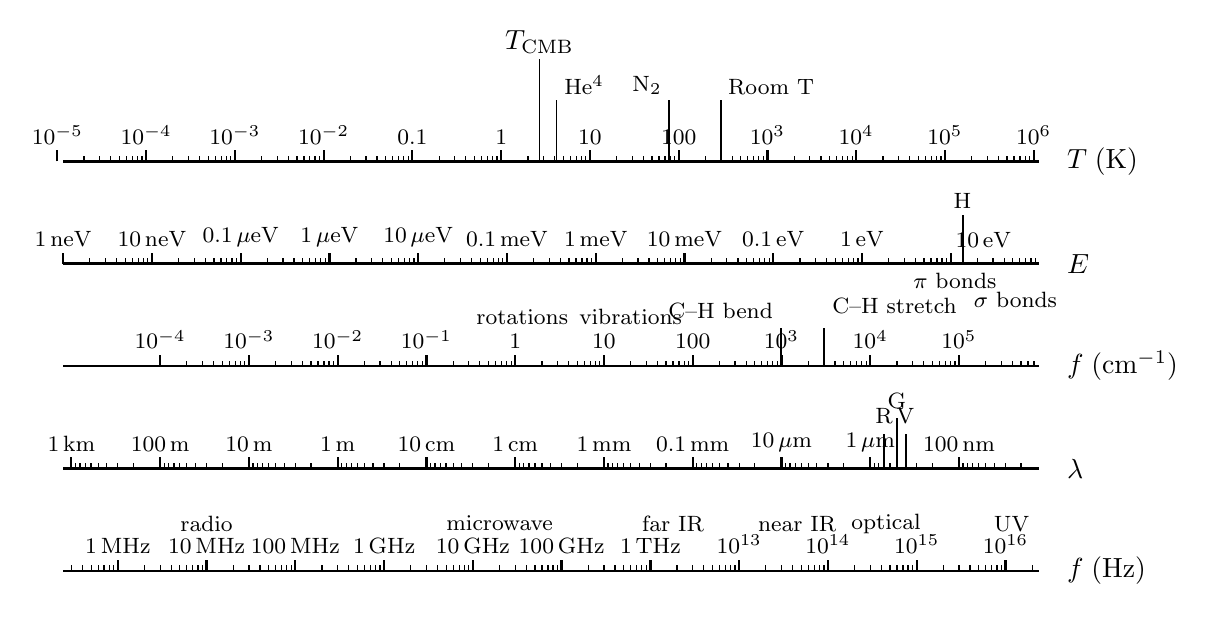
\begin{tikzpicture}[line width=0.8pt,>=Stealth,
  lab/.style={above,inner sep=1.5pt,font=\footnotesize}]
\draw[line width=0.9] (0,0) -- (12.4,0);
\foreach \xx/\l in {-0.073/{$10^{-5}$},1.054/{$10^{-4}$},2.182/{$10^{-3}$},3.309/{$10^{-2}$},4.436/{$0.1$},5.564/{$1$},6.691/{$10$},7.818/{$100$},8.945/{$10^{3}$},10.073/{$10^{4}$},11.200/{$10^{5}$},12.327/{$10^{6}$}}{
  \draw (\xx,0) -- ++(0,0.14);
  \node[lab] at (\xx,0+0.15) {\l};
}
\foreach \xx in {0.267,0.465,0.606,0.715,0.804,0.880,0.945,1.003,1.394,1.592,1.733,1.842,1.932,2.007,2.072,2.130,2.521,2.720,2.860,2.970,3.059,3.134,3.200,3.257,3.648,3.847,3.988,4.097,4.186,4.262,4.327,4.385,4.776,4.974,5.115,5.224,5.313,5.389,5.454,5.512,5.903,6.101,6.242,6.351,6.441,6.516,6.582,6.639,7.030,7.229,7.370,7.479,7.568,7.643,7.709,7.767,8.157,8.356,8.497,8.606,8.695,8.771,8.836,8.894,9.285,9.483,9.624,9.733,9.823,9.898,9.963,10.021,10.412,10.610,10.751,10.861,10.950,11.025,11.091,11.148,11.539,11.738,11.879,11.988,12.077,12.153,12.218,12.276}{
  \draw[line width=0.45] (\xx,0) -- ++(0,0.07);
}
\node[anchor=west] at (12.62,0) {$T\;(\mathrm{K})$};
\draw[line width=0.7] (6.050,0) -- ++(0,1.30);
\node[above,inner sep=1pt] at (6.050,1.32) {$T_{\mathrm{CMB}}$};
\draw[line width=0.7] (6.266,0) -- ++(0,0.78);
\node[lab,anchor=south west,inner sep=1pt] at (6.316,0.8) {$\mathrm{He}^4$};
\draw[line width=0.7] (7.690,0) -- ++(0,0.78);
\node[lab,anchor=south east,inner sep=1pt] at (7.650,0.8) {$\mathrm{N}_2$};
\draw[line width=0.7] (8.356,0) -- ++(0,0.78);
\node[lab,anchor=south west,inner sep=1pt] at (8.396,0.8) {Room T};
\draw[line width=0.9] (0,-1.3) -- (12.4,-1.3);
\foreach \xx/\l in {0.000/{$1\,$neV},1.127/{$10\,$neV},2.255/{$0.1\,\mu$eV},3.382/{$1\,\mu$eV},4.509/{$10\,\mu$eV},5.636/{$0.1\,$meV},6.764/{$1\,$meV},7.891/{$10\,$meV},9.018/{$0.1\,$eV},10.145/{$1\,$eV}}{
  \draw (\xx,-1.3) -- ++(0,0.14);
  \node[lab] at (\xx,-1.3+0.15) {\l};
}
\foreach \xx in {0.339,0.538,0.679,0.788,0.877,0.953,1.018,1.076,1.467,1.665,1.806,1.915,2.004,2.080,2.145,2.203,2.594,2.792,2.933,3.042,3.132,3.207,3.273,3.330,3.721,3.920,4.061,4.170,4.259,4.334,4.400,4.458,4.848,5.047,5.188,5.297,5.386,5.462,5.527,5.585,5.976,6.174,6.315,6.424,6.514,6.589,6.654,6.712,7.103,7.301,7.442,7.552,7.641,7.716,7.782,7.839,8.230,8.429,8.570,8.679,8.768,8.844,8.909,8.967,9.358,9.556,9.697,9.806,9.895,9.971,10.036,10.094,10.485,10.683,10.824,10.933,11.023,11.098,11.163,11.221,11.612,11.811,11.951,12.061,12.150,12.225,12.291,12.348}{
  \draw[line width=0.45] (\xx,-1.3) -- ++(0,0.07);
}
\node[anchor=west] at (12.62,-1.3) {$E$};
\draw (11.273,-1.3) -- ++(0,0.14);
\node[lab,anchor=south west,inner sep=1pt] at (11.285,-1.1500000000000001) {$10\,$eV};
\draw[line width=0.7] (11.423,-1.3) -- ++(0,0.62);
\node[lab] at (11.423,-0.66) {H};
\draw[line width=0.9] (0,-2.6) -- (12.4,-2.6);
\foreach \xx/\l in {1.233/{$10^{-4}$},2.360/{$10^{-3}$},3.487/{$10^{-2}$},4.614/{$10^{-1}$},5.742/{$1$},6.869/{$10$},7.996/{$100$},9.123/{$10^{3}$},10.251/{$10^{4}$},11.378/{$10^{5}$}}{
  \draw (\xx,-2.6) -- ++(0,0.14);
  \node[lab] at (\xx,-2.6+0.15) {\l};
}
\foreach \xx in {1.572,1.770,1.911,2.020,2.110,2.185,2.251,2.308,2.699,2.898,3.039,3.148,3.237,3.312,3.378,3.436,3.826,4.025,4.166,4.275,4.364,4.440,4.505,4.563,4.954,5.152,5.293,5.402,5.492,5.567,5.632,5.690,6.081,6.279,6.420,6.530,6.619,6.694,6.760,6.817,7.208,7.407,7.548,7.657,7.746,7.822,7.887,7.945,8.336,8.534,8.675,8.784,8.873,8.949,9.014,9.072,9.463,9.661,9.802,9.911,10.001,10.076,10.141,10.199,10.590,10.789,10.929,11.039,11.128,11.203,11.269,11.326,11.717,11.916,12.057,12.166,12.255,12.331}{
  \draw[line width=0.45] (\xx,-2.6) -- ++(0,0.07);
}
\node[anchor=west] at (12.62,-2.6) {$f\;(\mathrm{cm}^{-1})$};
\node[font=\footnotesize] at (5.831,-1.98) {rotations};
\node[font=\footnotesize] at (7.208,-1.98) {vibrations};
\draw[line width=0.7] (9.123,-2.6) -- ++(0,0.48);
\node[font=\footnotesize,anchor=south east,inner sep=1pt] at (9.063,-2.04) {C--H bend};
\draw[line width=0.7] (9.661,-2.6) -- ++(0,0.48);
\node[font=\footnotesize,anchor=south west,inner sep=1pt] at (9.721,-1.98) {C--H stretch};
\node[font=\footnotesize,anchor=south west,inner sep=1pt] at (10.749,-1.6600000000000001) {$\pi$ bonds};
\node[font=\footnotesize,anchor=south west,inner sep=1pt] at (11.519,-1.9000000000000001) {$\sigma$ bonds};
\draw[line width=0.9] (0,-3.9) -- (12.4,-3.9);
\foreach \xx/\l in {0.105/{$1\,$km},1.233/{$100\,$m},2.360/{$10\,$m},3.487/{$1\,$m},4.614/{$10\,$cm},5.742/{$1\,$cm},6.869/{$1\,$mm},7.996/{$0.1\,$mm},9.123/{$10\,\mu$m},10.251/{$1\,\mu$m},11.378/{$100\,$nm}}{
  \draw (\xx,-3.9) -- ++(0,0.14);
  \node[lab] at (\xx,-3.9+0.15) {\l};
}
\foreach \xx in {12.166,11.967,11.827,11.717,11.628,11.553,11.487,11.430,11.039,10.840,10.699,10.590,10.501,10.425,10.360,10.302,9.911,9.713,9.572,9.463,9.374,9.298,9.233,9.175,8.784,8.586,8.445,8.336,8.246,8.171,8.105,8.048,7.657,7.458,7.318,7.208,7.119,7.044,6.978,6.921,6.530,6.331,6.190,6.081,5.992,5.916,5.851,5.793,5.402,5.204,5.063,4.954,4.864,4.789,4.724,4.666,4.275,4.077,3.936,3.826,3.737,3.662,3.596,3.539,3.148,2.949,2.808,2.699,2.610,2.534,2.469,2.411,2.020,1.822,1.681,1.572,1.483,1.407,1.342,1.284,0.893,0.695,0.554,0.445,0.355,0.280,0.215,0.157}{
  \draw[line width=0.45] (\xx,-3.9) -- ++(0,0.07);
}
\node[anchor=west] at (12.62,-3.9) {$\lambda$};
\draw[line width=0.7] (10.425,-3.9) -- ++(0,0.44);
\node[lab] at (10.425,-3.4) {R};
\draw[line width=0.7] (10.699,-3.9) -- ++(0,0.44);
\node[lab] at (10.699,-3.4) {V};
\draw[line width=0.7] (10.590,-3.9) -- ++(0,0.64);
\node[lab] at (10.590,-3.2) {G};
\draw[line width=0.9] (0,-5.2) -- (12.4,-5.2);
\foreach \xx/\l in {0.695/{$1\,$MHz},1.822/{$10\,$MHz},2.950/{$100\,$MHz},4.077/{$1\,$GHz},5.204/{$10\,$GHz},6.331/{$100\,$GHz},7.459/{$1\,$THz},8.586/{$10^{13}$},9.713/{$10^{14}$},10.841/{$10^{15}$},11.968/{$10^{16}$}}{
  \draw (\xx,-5.2) -- ++(0,0.14);
  \node[lab] at (\xx,-5.2+0.15) {\l};
}
\foreach \xx in {0.106,0.246,0.356,0.445,0.520,0.586,0.643,1.034,1.233,1.374,1.483,1.572,1.648,1.713,1.771,2.162,2.360,2.501,2.610,2.700,2.775,2.840,2.898,3.289,3.487,3.628,3.738,3.827,3.902,3.968,4.025,4.416,4.615,4.756,4.865,4.954,5.030,5.095,5.153,5.544,5.742,5.883,5.992,6.081,6.157,6.222,6.280,6.671,6.869,7.010,7.119,7.209,7.284,7.349,7.407,7.798,7.997,8.137,8.247,8.336,8.411,8.477,8.534,8.925,9.124,9.265,9.374,9.463,9.539,9.604,9.662,10.053,10.251,10.392,10.501,10.590,10.666,10.731,10.789,11.180,11.378,11.519,11.628,11.718,11.793,11.859,11.916,12.307}{
  \draw[line width=0.45] (\xx,-5.2) -- ++(0,0.07);
}
\node[anchor=west] at (12.62,-5.2) {$f\;(\mathrm{Hz})$};
\node[font=\footnotesize] at (1.822,-4.6000000000000005) {radio};
\node[font=\footnotesize] at (5.544,-4.6000000000000005) {microwave};
\node[font=\footnotesize] at (7.746,-4.6000000000000005) {far IR};
\node[font=\footnotesize] at (9.322,-4.6000000000000005) {near IR};
\node[font=\footnotesize] at (10.450,-4.6000000000000005) {optical};
\node[font=\footnotesize,anchor=east] at (12.4,-4.6000000000000005) {UV};
\end{tikzpicture}
\end{document}
